\section{The Qutrit}
\subsection{Construction of the system}
In \cite{darkpath} a qubit is implemented by modifying the lambda system, adding an additional level, an auxiliary state, effectively turning it into a tripod. 
The generalization to implement a qutrit is not trivial but it is clear that one extra ground state is required to make the computational basis larger. Another thing that is needed is to limit the number of dark states to one. The number of dark states is the difference of number of exited states and the number of ground states\cite{lambda} (here the auxiliary state is \textbf{not} counted as a ground state). Therefor another excited state must be added as well. How these state are coupled is the hard part, we will see that the system given by the Hamiltonian
\begin{equation}
\label{eq:Ham}
H = \sum_{j = 1}^2 \sum_{i =j}^{3} \omega_{ij}\ket{i}\bra{e_j}  + \frac{\Omega_{a}(t)}{2}\ket{a}\bra{e_2}  +\,\text{h.c}
\end{equation}
which is shown in Figure \ref{fig:Ham}, will work.  It consists of two excited states, $\ket{e_1}, \ket{e_2}$, an auxiliary state $\ket{a}$ and the ground states $\ket{1}, \ket{2}, \ket{3}$ which 
makes up the computational basis of the qutrit. By changing the basis of the Hamiltonian, it can be rewritten as 
\begin{equation}
\label{eq:Hamd}
H_d = \sum_{j = 1}^2 \frac{\Omega_j(t)}{2}e^{-i\phi_j}\ket{b_j}\bra{e_j}  + \frac{\Omega_a(t)}{2}\ket{a}\bra{e_2}  +\,\text{h.c}
\end{equation} 
by a Morris-Shore transformation\cite{morris}. We call this new basis the dark state basis. To find this basis find a dark state to the original  Hamiltonian, an eigenstate with eigenvalue $0$, $H\ket{d} = 0$, then find two bright states, orthogonal to both $\ket{d}$ and each other. This basis can be parametrized with 4 angles, $\theta, \varphi, \chi, \xi$, the dark state is on the form $\ket{d} = \cos\theta\ket{1} + e^{i\chi}\sin\theta\cos\varphi\ket{2} + e^{i\xi}\sin\theta\sin\varphi\ket{3}$, additionally the two bright states are $\ket{b_1} = N_1 \left(-e^{i\xi}\sin\theta\sin\varphi\ket{1} + \cos\theta\ket{2} \right)$ and $\ket{b_2} = N_2 \left(\cos\theta\ket{1} +  e^{i\chi}\sin\theta\cos\varphi\ket{2} + \Lambda \ket{3}\right ) $, where $N_1, N_2$ are normalization factors and $\Lambda$ can be chosen such that $\bra{d}\ket{b_2} = 0$.

\begin{figure}[H]
\label{fig:Ham}
    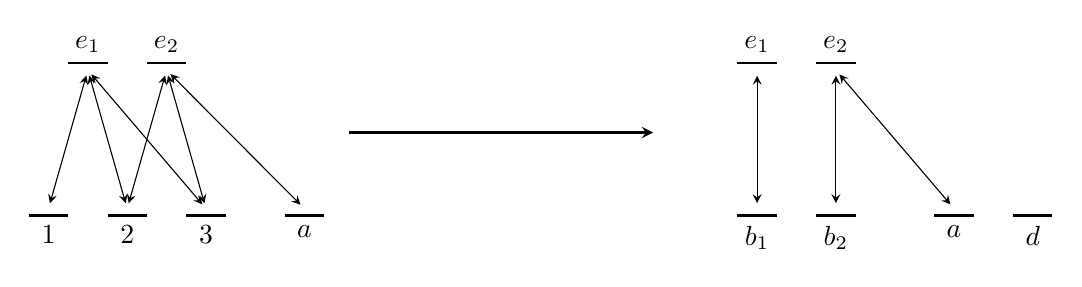
\begin{tikzpicture}[
      scale=0.5,
      level/.style={thick},
      virtual/.style={thick,densely dashed},
      trans/.style={thin,<->,shorten >=2pt,shorten <=2pt,>=stealth},
      arrow/.style={thick,->,shorten >=2pt,shorten <=2pt,>=stealth},
      classical/.style={thin,double,<->,shorten >=4pt,shorten <=4pt,>=stealth}]
      
    % Excited
    \draw[level] (5cm,0em) -- (6cm,0em) node[midway,above] {$\ket{e_1}$};    
    \draw[level] (7cm,0em) -- (8cm,0em) node[midway,above] {$\ket{e_2}$};
	% Ground states
    \draw[level] (4cm,-11em) -- (5cm,-11em) node[midway,below] {$\ket{1}$};
    \draw[level] (6cm,-11em) -- (7cm,-11em) node[midway,below] {$\ket{2}$};
    \draw[level] (8cm,-11em) -- (9cm,-11em) node[midway,below] {$\ket{3}$};
    \draw[level] (10.5cm,-11em) -- (11.5cm,-11em) node[midway,below] {$\ket{a}$};
    % e_1
    % Draw the transitions.
    \draw[trans] (5.5cm,-0.5em) -- (4.5cm,-10.5em) node[midway,left] {};
    \draw[trans] (5.5cm,-0.5em) -- (6.5cm,-10.5em) node[midway,left] {};
    \draw[trans] (5.5cm,-0.5em) -- (8.5cm,-10.5em) node[midway,left] {};
   	% e_2
    \draw[trans] (7.5cm,-0.5em) -- (6.5cm,-10.5em) node[midway,left] {};
    \draw[trans] (7.5cm,-0.5em) -- (8.5cm,-10.5em) node[midway,left] {};
    \draw[trans] (7.5cm,-0.5em) -- (11cm,-10.5em) node[midway,left] {};
    
    \draw[arrow] (12cm,-5em) -- (20cm,-5em) node[] {}; 
    
    % Excited
    \draw[level] (22cm,0em) -- (23cm,0em) node[midway,above] {$\ket{e_1}$};    
    \draw[level] (24cm,0em) -- (25cm,0em) node[midway,above] {$\ket{e_2}$};
    \draw[level] (22cm,-11em) -- (23cm,-11em) node[midway,below] {$\ket{b_1}$};
    \draw[level] (24cm,-11em) -- (25cm,-11em) node[midway,below] {$\ket{b_2}$};
    \draw[level] (27cm,-11em) -- (28cm,-11em) node[midway,below] {$\ket{a}$};
    \draw[level] (29cm,-11em) -- (30cm,-11em) node[midway,below] {$\ket{d}$};
    
  	\draw[trans] (22.5cm,-0.5em) -- (22.5cm,-10.5em) node[midway,left] {};
	\draw[trans] (24.5cm,-0.5em) -- (24.5cm,-10.5em) node[midway,left] {};
	\draw[trans] (24.5cm,-0.5em) -- (27.5cm,-10.5em) node[midway,left] {};
    \end{tikzpicture}    
    \caption{The system given by the Hamiltonian shown in Equation \ref{eq:Ham} (left) and the transformed system from Equation \ref{eq:Hamd} (right)} 
\end{figure}

These states are bright states which will make up a new orthonormal basis. 
Explicitly the states are 
\begin{equation}
\label{eq:states}
\begin{aligned}
\ket{d} &= \cos\theta\ket{1} + e^{i\chi}\sin\theta\cos\varphi\ket{2} + e^{i\xi}\sin\theta\sin\varphi\ket{3}
\\
\ket{b_1} &= \frac{1}{\sqrt{1-\sin^2\theta\sin^2\varphi}} \left(-e^{-i\chi}\sin\theta\cos\varphi\ket{1} + \cos\theta\ket{2} \right)
\\
\ket{b_2} &= \frac{1}{\sqrt{1-\sin^2\theta\sin^2\varphi}} \left(\sin\theta\sin\varphi\cos\theta\ket{1} + \dfrac{e^{i\chi}}{2}\sin^2\theta\sin 2\varphi\ket{2} + e^{i\xi}(\sin^2\theta\sin^2\varphi - 1)\ket{3}\right)
\end{aligned}
\end{equation}
The parameters $\omega_{ij}$ in the original basis can be determined by replacing the states in $H_d$ by their form in the $\{\ket{1},\ket{2},\ket{3}\}$ basis.

Now lets introduce the concept of a dark path, $\bra{D(t)}H_d\ket{D(t)} = 0$, along this path the average energy is always zero. Thus no dynamical phase is accumulated during the time evolution and therefor it follows the conditions required for NHQC.

The following two states satisfy the dark path condition and can be parametrized by two angles $u(t), v(t)$.
\begin{equation}
\label{eq:dpaths}
\begin{aligned}
\ket{D_1(t)} &= \cos u e^{-i\phi_1}\ket{b_1} + i\sin u \ket{e_1}
\\
\ket{D_2(t)} &= \cos u\cos v e^{-i\phi_2}\ket{b_2} - i\sin u \ket{e_2} - \cos u\sin v \ket{a}
\end{aligned}
\end{equation}
it can easily be verified that $\bra{D_i(t)}H_d\ket{D_j(t)} = 0, i,j = 1,2$. The angles can be chosen with the constraint that the boundary condition $\ket{D_i(0)}\bra{D_i(0)} = \ket{D_i(T)}\bra{D_i(T)}, i = 1,2$. This can be achieved by choosing $u(0) = u(T) = v(0) = v(T) = 0$. A valid choice is $u(t) = \frac{\pi}{2}\sin^2\frac{\pi t}{T}$ and $v(t) = \eta\left[1 - \cos u(t)\right]$, as for the 2D case. Unless mentioned otherwise $\eta = 4.0$. Each dark path starts in the respective bright state and travels along a curve and then returns to the bright state. The choice 

Using the Schrödinger equation one can relate the dark path to the Hamiltonian,
\begin{equation}
i\pdv{}{t}\ket{D_i(t)} = H_d\ket{D_i(t)},
\end{equation}
and thusly one can reverse engineer the time dependent parameters $\Omega_i(t)$ by matching the factors of states. A calculation yields 
\begin{equation}
\begin{aligned}
\Omega_1(t) &= -2\dot{u}
\\ 
\Omega_2(t) &= 2\left(\dot{v}\cot u\sin v + \dot{u}\cos v \right)
\\
\Omega_a(t) &= 2\left(\dot{v}\cot u\cos v - \dot{u}\sin v \right).
\end{aligned}
\end{equation}

To construct a quantum gate, we make use of the method of multi-pulse single-loops\cite{sLoop}, the relevant part of the time evolution operator is
\begin{equation}
\begin{aligned}&
U_1 = \ket{d}\bra{d} -i\ket{e_1}\bra{b_1} -i\ket{e_2}\bra{b_2},\; \phi_1 = \phi_2 = 0
\\&
U_2 = \ket{d}\bra{d} +ie^{i\gamma_1}\ket{b_1}\bra{e_1} +ie^{i\gamma_2}\ket{b_2}\bra{e_2},\; \phi_1 = -\gamma_1,\; \phi_2 = -\gamma_2
\end{aligned}
\end{equation}
so the operator for one full loop is 
\begin{equation}
\label{eq:trit-gate-1-loop}
U = U_2U_1 = \ket{d}\bra{d} + e^{i\gamma_1}\ket{b_1}\bra{b_1} + e^{i\gamma_2}\ket{b_2}\bra{b_2}.
\end{equation}
This transformation can be parametrized by $6$ real parameters, $U(\chi,\xi,\theta,\varphi,\gamma_1,\gamma_2)$, however it is not enough to construct all gates, for example $X_3$ requires 2 loops. This is since one loop does not cover all degrees of freedom. The reason for this is elaborated on later in the Generalization section. So the full gate is given by repeating $U$ with another set of parameters. So the full gate $\mathbb{U}$ is given by 
\begin{equation}
\label{eq:trit-gate-2-loop}
\mathbb{U} = U(\chi',\xi',\theta',\varphi',\gamma_1',\gamma_2') U(\chi,\xi,\theta,\varphi,\gamma_1,\gamma_2)
\end{equation}
Now the problem is only a matter of finding all parameters to replicate the desired gate. This is a non-trivial problem since it include solving a system of 9 non-linear equation containing 12 variables for a gate requiring two loops. Some gates that only require a single loop can with some work be found analytically but the problem quickly becomes too complex to handle.

\subsection{Implementation}
The implementation is quite straight forward, for given set of parameters, say that we want to see how the initial state $\ket{\psi(0)}$ evolves with time.
Let $\ket{\psi(0)} = (a,b,c)^T$ in the computational basis $\{\ket{1},\ket{2},\ket{3}\}$. Then the following equation can be formulated, for some coefficients $f_i$,
\begin{equation}
\begin{pmatrix}
a\\
b\\
c
\end{pmatrix}
= f_0 \ket{d} + f_1\ket{b_1} + f_2\ket{b_2}
\end{equation}
since at time $t = 0$ the dark paths are in the corresponding bright state.
Now expand the dark state and bright state in terms of the original basis. Doing this one can obtain the relation
\begin{equation}
\begin{pmatrix}
f_0\\
f_1\\
f_2
\end{pmatrix} = \begin{pmatrix}
c_1 & -N_1 c_2 & N_2 c_1
\\
c_2 & N_1 c_1 & N_2 c_2
\\
c3 & 0 & N_2 \Lambda
\end{pmatrix}^{-1}\begin{pmatrix}
a\\
b\\
c
\end{pmatrix}
\end{equation}
So by choosing an initial state, the coefficients can be obtained.
Then the system can be solved for any time $t \in T$ using Equation 
\begin{equation}
\label{eq:expl-time}
\ket{\psi(t)} = f_0\ket{d} + f_1\ket{D_1(t)} + f_2\ket{D_2(t)}, t \in [0,T].
\end{equation}
To see the effect of the gates, the probability of finding the system in the standard computational basis states can be plotted against time to see how the gate transform the state from initial to final state, shown in Figure \ref{fig:pop_X} and \ref{fig:pop_H} for the $X_3$ and $H_3$ gates respectively . 
\begin{figure}[H]
\label{fig:pop_X}
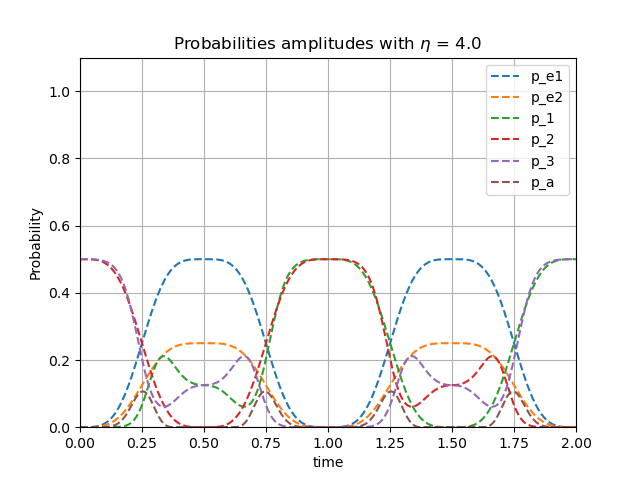
\includegraphics[scale=0.5]{figures/pop_plot_X011.png}
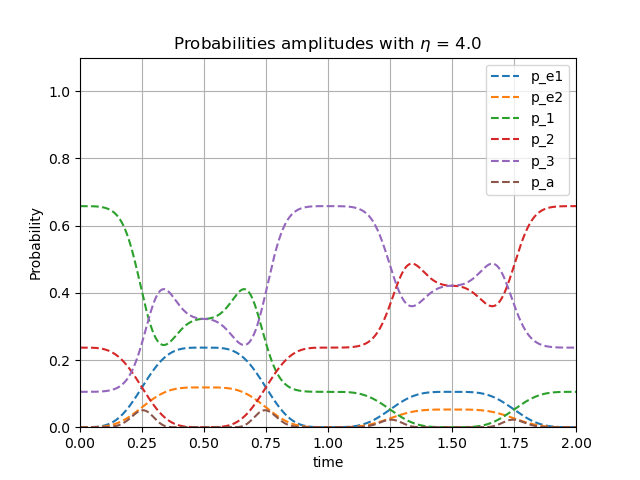
\includegraphics[scale=0.5]{figures/pop_plot_X532.png}
\caption{The effect of the $X_3$-gate on the initial states $\dfrac{1}{\sqrt{2}}[0,1,1]$ (left) and $\dfrac{1}{\sqrt{33}}[5,3,2]$ (right). Note that since the plot shows the probabilities, phases can not be seen in the plot.}
\end{figure}

\begin{figure}[H]
\label{fig:pop_H}
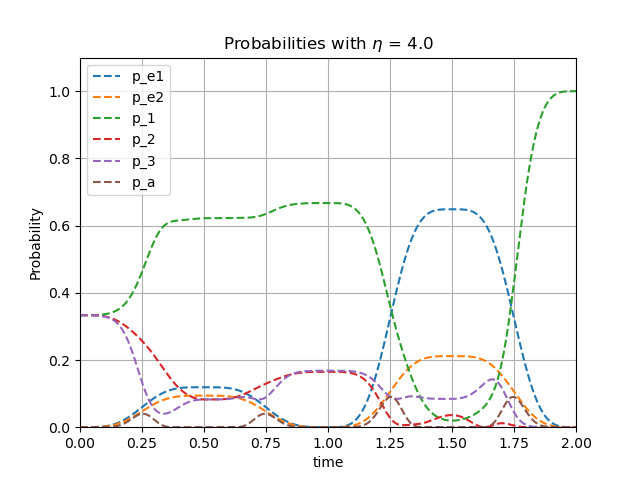
\includegraphics[scale=0.5]{figures/pop_plot_H111.png}
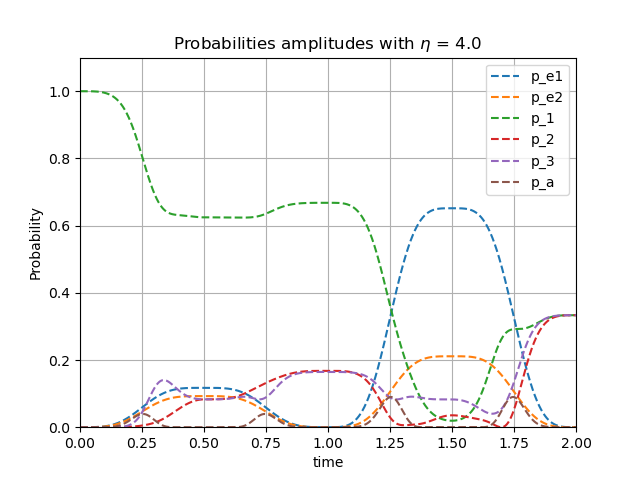
\includegraphics[scale=0.5]{figures/pop_plot_H100.png}
\caption{The effect of the $H_3$-gate on the initial states $\dfrac{1}{\sqrt{3}}[1,1,1]$ (left) and $[1,0,0]$ (right). Note that since the plot shows the probabilities, phases can not be seen in the plot.}
\end{figure}


\subsection{Important gates, Universality and parameter selection}
By specifying the parameters of $U$ the qutrit gates from the Background section can be constructed, a selection of important gates are obtained by the following;
\begin{equation}
\begin{aligned}
X_3 &= U(0,0,\dfrac{\pi}{4},\dfrac{\pi}{2},0,\pi)U(0,0,\dfrac{\pi}{2},\dfrac{\pi}{4},0,\pi) 
= \begin{pmatrix}
0&0&1
\\
1&0&0
\\
0&1&0
\end{pmatrix}
\\ 
Z_3 &= U(0,0,0,0,\dfrac{2\pi}{3},\dfrac{4\pi}{3})
= \begin{pmatrix}
1&0&0
\\
0&e^{\frac{2\pi i}{3}}&0
\\
0&0&e^{\frac{4\pi i}{3}}
\end{pmatrix}
\\
T_3 &= U(0,0,0,0,\dfrac{2\pi}{9},\dfrac{-2\pi}{9})
= \begin{pmatrix}
1&0&0
\\
0&e^{\frac{2\pi i}{9}}&0
\\
0&0&e^{\frac{-2\pi i}{9}}
\end{pmatrix}
\\
H_3 &= U(6.41010859\cdot 10^{-4}, 6.55568952\cdot 10^{-4}, .475667128, .785362474, 1.58054108, 1.56302702)\\ \times &U(9.81289849\cdot 10^{-3}, 3.56878815\cdot 10^{-18},1.18743379, 2.15063745, 9.74301696\cdot 10^{-17}, 1.56882773)\\
&\approx \dfrac{1}{\sqrt{3}}\begin{pmatrix}
1&1&1
\\
1&e^{\frac{2\pi i}{3}}&e^{\frac{4\pi i}{3}}
\\
1&e^{\frac{4\pi i}{3}}&e^{\frac{2\pi i}{3}}
\end{pmatrix}.
\end{aligned}
\end{equation}
Note that the choice of parameters are not unique and there are multiple ways to create the same unitary. These gates are enough to achieve single-qutrit universality as discussed in Section Theoretical Background. To achieve full universality an additional two-qutrit gate is needed. A common choice for qubits is the {\tt CNOT} gate\cite{qudit}.

The parameters for a given gate can be specified by solving the non-linear system of equations obtained from by setting the matrix representation of the gate equal to Equation \ref{eq:trit-gate-1-loop} or \ref{eq:trit-gate-2-loop}. For the diagonal gates the analytical solution can be easily found by fixing $\theta = \varphi = \chi = \xi = 0$ the basis states reduce to $\ket{d} = \ket{1}, \ket{b_1} = \ket{2}, \ket{b_2} = -\ket{3}$, then all diagonal unitaries can be specified by $\gamma_1$ and $\gamma_2$ up to a phase factor,
\begin{equation}
U(0,0,0,0,\gamma_1,\gamma_2) = \begin{pmatrix}
1&0&0
\\
0&e^{i\gamma_1}&0
\\
0&0&e^{i\gamma_2}
\end{pmatrix}.
\end{equation}

Analytical solutions are not always easy to find, the $H_3$-gate gives rise to a system of equation that is non-trivial to solve. In that case an approximative gate $\tilde{U}$ can be found by numerical optimization of the expression $\text{min}||U-\tilde{U}||_F$, where $||\cdot||_F$ is the Frobenius matrix \note{some citation maybe?} norm given by $||A||_F = \sqrt{\text{Tr}\left[A^\dagger A \right]}$. Since $\tilde{U} \approx U$ the approximated gates effect will be very close to that of the exact gate.

To assess the robustness of the gate the fidelity is used, a metric that measures how close two quantum states are to each other, $F(\ket{\psi},\ket{\varphi}) = |\bra{\psi}\ket{\varphi}|$. The fidelity is averaged by sampling initial states and letting them evolve  with time (numerically solving the Schrödinger Equation), and then comparing to the exact solution obtained by multiplying the gate with the initial state. The calculated fidelities are shown in Figure \ref{fig:fidelity}. 

\begin{figure}[H]
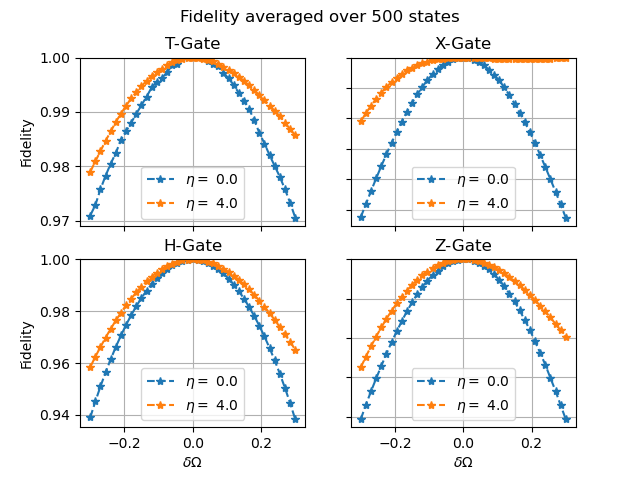
\includegraphics[scale=1]{figures/Fid500.png}

\caption{Robustness test, average fidelity of the $T_3,X_3,Z_3,$ and $H_3$ gates. Average calculated by sampling over 500 randomized initial states with a perturbation of the $\Omega$-pulses, $\Omega \mapsto \Omega(1+\delta)$ .}
\label{fig:fidelity}
\end{figure}


\newpage
\section{Generalization}
To generalize the scheme to a qudit with arbitrary dimension $n$,  the same idea from the qutrit case can be extended, $n$ ground states, $m = n - 1$ excited states and 1 auxiliary state, there for the dimension of the Hilbert space is  $n + m + 1 = n + 1 -1 = 2n$. Once again the couplings are not trivial and will be somewhat intricate, but the couplings given by the Hamiltonian in Equation \ref{eq:HamN}, will do the trick. 

\begin{equation}
H = \sum_{j = 1}^m \sum_{i = j}^n \omega_{ij} \ket{i}\bra{e_j} + \frac{\Omega_a(t)}{2}\ket{a}\bra{e_m} +\;\text{h.c}
\label{eq:HamN}
\end{equation}

\begin{figure}[H]
    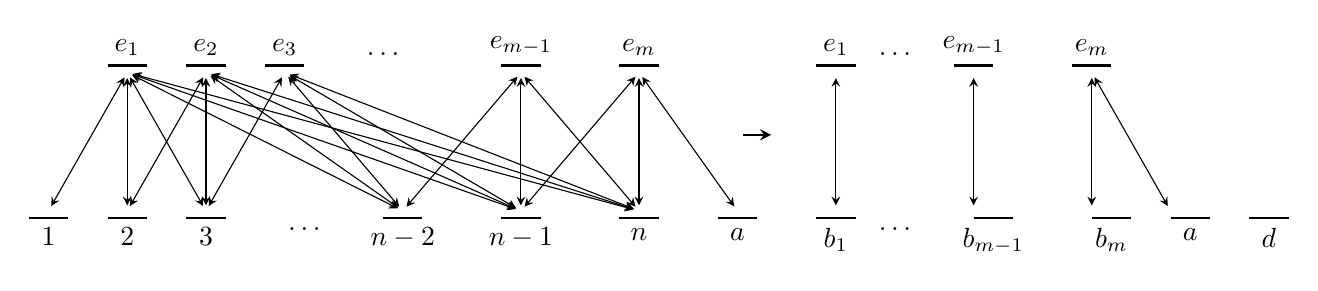
\begin{tikzpicture}[
      scale=0.5,
      level/.style={thick},
      virtual/.style={thick,densely dashed},
      trans/.style={thin,<->,shorten >=2pt,shorten <=2pt,>=stealth},
      arrow/.style={thick,->,shorten >=2pt,shorten <=2pt,>=stealth},
      classical/.style={thin,double,<->,shorten >=4pt,shorten <=4pt,>=stealth}]
    \draw[level] (4cm,-11em) -- (5cm,-11em) node[midway,below] {$\ket{1}$};
    \draw[level] (6cm,-11em) -- (7cm,-11em) node[midway,below] {$\ket{2}$};
    \draw[level] (8cm,-11em) -- (9cm,-11em) node[midway,below] {$\ket{3}$};
    \draw (11cm,-11em)  node[below] {$\dots$}; 
    \draw[level] (13cm,-11em) -- (14cm,-11em) node[midway,below] {$\ket{n-2}$};
    \draw[level] (16cm,-11em) -- (17cm,-11em) node[midway,below] {$\ket{n-1}$};
    \draw[level] (19cm,-11em) -- (20cm,-11em) node[midway,below] {$\ket{n}$};
    \draw[level] (21.5cm,-11em) -- (22.5cm,-11em) node[midway,below] {$\ket{a}$}; 
  % Draw the energy levels.
    \draw[level] (6cm,0em) -- (7cm,0em) node[midway,above] {$\ket{e_1}$};    
   	\draw[level] (8cm,0em) -- (9cm,0em) node[midway,above] {$\ket{e_2}$};
   	\draw[level] (10cm,0em) -- (11cm,0em) node[midway,above] {$\ket{e_3}$};
    \draw (13cm, 0em) node[above] {$\dots$}; 
    \draw[level] (16cm,0em) -- (17cm,0em) node[midway,above] {$\ket{e_{m-1}}$};
    \draw[level] (19cm,0em) -- (20cm,0em) node[midway,above] {$\ket{e_{m}}$};
    % Draw the transitions.
   % e_1
    \draw[trans] (6.5cm,-0.5em) -- (4.5cm,-10.5em) node[midway,left] {};
    \draw[trans] (6.5cm,-0.5em) -- (6.5cm,-10.5em) node[midway,left] {};
    \draw[trans] (6.5cm,-0.5em) -- (8.5cm,-10.5em) node[midway,left] {};
    \draw[trans] (6.5cm,-0.5em) -- (13.5cm,-10.5em) node[midway,left] {};
	\draw[trans] (6.5cm,-0.5em) -- (16.5cm,-10.5em) node[midway,left] {};
    \draw[trans] (6.5cm,-0.5em) -- (19.5cm,-10.5em) node[midway,left] {};       
   % e_2
    \draw[trans] (8.5cm,-0.5em) -- (6.5cm,-10.5em) node[midway,left] {};
    \draw[trans] (8.5cm,-0.5em) -- (8.5cm,-10.5em) node[midway,left] {};
    \draw[trans] (8.5cm,-0.5em) -- (13.5cm,-10.5em) node[midway,left] {};
	\draw[trans] (8.5cm,-0.5em) -- (16.5cm,-10.5em) node[midway,left] {};
    \draw[trans] (8.5cm,-0.5em) -- (19.5cm,-10.5em) node[midway,left] {};
    % e_3
    \draw[trans] (10.5cm,-0.5em) -- (8.5cm,-10.5em) node[midway,left] {};
    \draw[trans] (10.5cm,-0.5em) -- (13.5cm,-10.5em) node[midway,left] {};
	\draw[trans] (10.5cm,-0.5em) -- (16.5cm,-10.5em) node[midway,left] {};
    \draw[trans] (10.5cm,-0.5em) -- (19.5cm,-10.5em) node[midway,left] {};
	% e_m-1
	\draw[trans] (16.5cm,-0.5em) -- (13.5cm,-10.5em) node[midway,left] {};
	\draw[trans] (16.5cm,-0.5em) -- (16.5cm,-10.5em) node[midway,left] {};
   	\draw[trans] (16.5cm,-0.5em) -- (19.5cm,-10.5em) node[midway,left] {};
	% e_m
	\draw[trans] (19.5cm,-0.5em) -- (16.5cm,-10.5em) node[midway,left] {};
   	\draw[trans] (19.5cm,-0.5em) -- (19.5cm,-10.5em) node[midway,left] {};   			 
   	\draw[trans] (19.5cm,-0.5em) -- (22cm,-10.5em) node[midway,left] {};
   	
   	
   	
   	 \draw[arrow] (22cm,-5em) -- (23cm,-5em) node[] {}; 
   	
   	\draw[level] (24cm,-11em) -- (25cm,-11em) node[midway,below] {$\ket{b_1}$};
    \draw (26cm,-11em)  node[below] {$\dots$};    
    \draw[level] (28cm,-11em) -- (29cm,-11em) node[midway,below] {$\ket{b_{m-1}}$};
    \draw[level] (31cm,-11em) -- (32cm,-11em) node[midway,below] {$\ket{b_m}$};
    \draw[level] (33cm,-11em) -- (34cm,-11em) node[midway,below] {$\ket{a}$};
    \draw[level] (35cm,-11em) -- (36cm,-11em) node[midway,below] {$\ket{d}$};
    
  % Draw the energy levels.
    \draw[level] (24cm,0em) -- (25cm,0em) node[midway,above] {$\ket{e_1}$};    
    \draw (26cm, 0em) node[above] {$\dots$};
    \draw[level] (27.5cm,0em) -- (28.5cm,0em) node[midway,above] {$\ket{e_{m-1}}$};
    \draw[level] (30.5cm,0em) -- (31.5cm,0em) node[midway,above] {$\ket{e_{m}}$};
        
    % Draw the transitions.
   % e_1
    \draw[trans] (24.5cm,-0.5em) -- (24.5cm,-10.5em) node[midway,left] {};     
	% e_m-1
	\draw[trans] (28cm,-0.5em) -- (28cm,-10.5em) node[midway,left] {};
	% e_m
	\draw[trans] (31cm,-0.5em) -- (31cm,-10.5em) node[midway,left] {};
	\draw[trans] (31cm,-0.5em) -- (33cm,-10.5em) node[midway,left] {};
    \end{tikzpicture}
    \caption{The system given by the Hamiltonian shown in Equation \ref{eq:HamN} (left) and the transformed system from Equation \ref{eq:HamdN} (right)}
    \label{fig:HamN}
\end{figure}



The general system for a qudit is given by $m$ excited states $\ket{e_i},\,i = 0,1,\dots,m$ and $n$ ground states labeled $\ket{i},\,i = 1,2,\dots,n$ and one auxiliary state $\ket{a}$. The number of states always follows that $n-m = 1$ to limit the number of dark states to one\cite{lambda}.
The transitions occur only between excited states and ground states. The couplings follow a pattern, the first excited state $e_1$ is connected to all ground states, $e_2$ is connected to all ground states except $\ket{1}$, in general the excited state $\ket{e_i}$ is connected to the $(n - i)$th ground states with the highest label. Unless $i = m$, the excited state $\ket{e_m}$ which is connected to the two highest labeled ground states and the auxiliary state $\ket{a}$. See Equation \ref{eq:HamN} and Figure \ref{fig:HamN} for a clarification. 

From the standard basis $\{e_1,e_2,\dots,e_m,1,2,\dots,n,a\}$, it is possible define a new basis, the dark state basis given by $\{e_1,e_2,\dots,e_m,b_1,b_2,\dots,b_{m},a,d\}$.

Assume a dark state on the form 
\begin{equation}
\ket{d} = c_1\ket{1} + c_2\ket{2} + c_3\ket{3} \dots + c_{n}\ket{n},\, |c_1|^2 + |c_2|^2 + \dots + |c_{n}|^2 = 1
\end{equation}
from this dark state one could recursively define $n-1 = m$ bright states.
Starting from
\begin{equation}
\ket{b_1} = N_1\left(-c_2\ket{1} + c_1\ket{2}\right)
\end{equation}
with $N_1$ being a normalization factor. Then choose additional bright states on the form
\begin{equation}
\begin{aligned}
&\ket{b_2} &=& N_2 \left(c_1\ket{1} + c_2\ket{2} + \Lambda_{1}^{(2)}\ket{3}  \right)
\\
&\ket{b_3} &=&  N_3 \left(c_1\ket{1} + c_2\ket{2} + \Lambda_{1}^{(3)}\ket{3} + \Lambda_{2}^{(3)}\ket{4} \right)
\\
&\;\;\vdots
\\
&\ket{b_{m-1}} &=& N_{m-1} \left( c_1\ket{1} + c_2\ket{2} + \Lambda_{1}^{(m-1)}\ket{2} + \Lambda_{2}^{(m-1)}\ket{3} + \dots + \Lambda_{m-2}^{(m-1)}\ket{m-1} \right)
\\
&\ket{b_{m}} &=& N_m \left( c_1\ket{1} + c_2\ket{2} + \Lambda_{1}^{(m)}\ket{2} + \Lambda_{2}^{(m)}\ket{3} + \dots + \Lambda_{m-2}^{(m)}\ket{m-1} + \Lambda_{m-1}^{(m)}\ket{m} \right).
\end{aligned}
\end{equation}
By this construction it is clear that $\ket{b_1}$ is orthogonal to all other bright states.

The coefficients can be chosen in such a way that, in $\ket{b_2}$, the coefficient $\Lambda_1^{(2)}$ can be chosen such that, $\bra{d}\ket{b_2} = 0$, and in $\ket{b_3}$, the coefficient $\Lambda_1^{(3)}$ can be chosen such that, $\bra{b_2}\ket{b_3} = 0$ and $\Lambda_2^{(3)}$ such that $\bra{d}\ket{b_3} = 0$. By recursively repeating this argument one could see that it is possible to chose $m$ bright states, then by normalizing all the $N_i$ can be found, thus we have obtained $m$ orthonormal bright states, $\bra{b_i}\ket{b_j} = \delta_{ij}$.
The coefficients $c_i$ can be parametrized by the euclidean components of the unit-$n$-sphere and a phase factor.

\begin{equation}
\begin{aligned}
c_1 &= \cos(\varphi_1)
\\ 
c_2 &= e^{i\theta_1}\sin(\varphi_1)\cos(\varphi_2)
\\ 
c_3 &= e^{i\theta_2}\sin(\varphi_1)\sin(\varphi_2)\cos(\varphi_3)
\\
&\hspace{2mm}\vdots
\\
c_{n-1} &= e^{i\theta_{n-1}}\sin(\varphi_1)\dots\sin(\varphi_{n-2})\cos(\varphi_{n-1})
\\
c_{n} &= e^{i\theta_{n}}\sin(\varphi_1)\dots\sin(\varphi_{n-2})\sin(\varphi_{n-1})
\end{aligned}
\end{equation}

$c_1$ does not need a phase factor since the overall phase of a state is non-measurable and can be chosen such that the first phase factor can be canceled. The remaining $\Lambda$ coefficients can be expressed in terms of the $c_i$.

In this newly defined space the Hamiltonian can be written as
\begin{equation}
H_d = \sum_{i = 1}^m \frac{\Omega_i(t)}{2}e^{-i\phi_i}\ket{b_i}\bra{e_i} + \frac{\Omega_a(t)}{2}\ket{a}\bra{e_n} +\;\text{h.c}
\label{eq:HamdN}
\end{equation}
with $\Omega_i$ being real-valued time dependent parameters and the $\phi_i$ time independent phase factors.

With this Hamiltonian $m$ dark paths can be constructed, and must satisfy $\bra{D_i(t)}H_d\ket{D_i(t)} = 0, i = 1,2,\dots,m$ and $\bra{D_i(t)}\ket{D_j(t)} = \delta_{ij}$.\\
The dark paths can be parametrized by two functions $u(t),v(t)$ that satisfy the conditions $u(0) = v(0) = u(T) = v(T) = 0$,  will have the form
\begin{equation}
\begin{aligned}
\ket{D_i(t)} &= \cos u e^{-i\phi_i}\ket{b_i} + i\sin u \ket{e_i},\, i = 1,2,\dots,m-1
\\
\ket{D_m(t)} &= \cos u \cos v e^{-i\phi_n}\ket{b_m} - i\sin u \ket{e_m} - \cos u \sin v \ket{a}
\end{aligned}
\end{equation}
The dark paths start in the bright state and travels along a curve where the expectation value of the energy is constantly $0$ and can thus be used non-adiabatically.

By using these states one can reverse engineer the Hamiltonian using the Schrödinger equation to determine $\Omega_i$ and $\Omega_a$ since 
\begin{equation}
i\pdv{}{t}\ket{D_i(t)} = H_d\ket{D_i(t)},\; i = 1,2,\dots,m
\end{equation}
a calculation yields
\begin{equation}
\begin{aligned}
\Omega_1(t) &= -2\dot{u}
\\ 
\Omega_2(t) &= -2\dot{u}
\\
&\hspace{2mm}\vdots
\\
\Omega_{m-1}(t) &= -2\dot{u}
\\
\Omega_m(t) &= 2\left(\dot{v}\cot u\sin v + \dot{u}\cos v \right)
\\
\Omega_a(t) &= 2\left(\dot{v}\cot u\cos v - \dot{u}\sin v \right)
\end{aligned}
\end{equation}

The time evolution is split into $k$ loops, each loop with two pulses, $0 \longrightarrow T/2$ and $T/2 \longrightarrow T$. The relevant part of the time evolution operator for one loop is  
$U_1(T/2,0) = \ket{d}\bra{d} -i\sum_{i = 1}^m \ket{e_i}\bra{b_i},\, \phi_i = 0, i = 1,2,\dots,n$ and $U_2(T,T/2) = \ket{d}\bra{d} + i\sum_{i = 1}^m e^{i\gamma_i}\ket{b_i}\bra{e_i},\, \phi_i = 0, i = 1,2,\dots,n $
The full operator for one loop is then given by 
\begin{equation}
U = U_2U_1 = \ket{d}\bra{d} + \sum_{i = 1}^{m}e^{i\gamma_i}\ket{b_i}\bra{b_i}.
\end{equation}
It is clear that $U$ is unitary in the subspace $\{d,b_1,b_2,\dots,b_n\}$

The unitary is parametrized by $3m = 3(n-1), n\geq 2$, parameters,
\begin{equation}
U(\varphi_1,\dots,\varphi_m,\theta_1,\dots,\theta_m,\gamma_1,\dots,\gamma_m) 
\end{equation} 

\note{The following part might not be 100\% correct, procced with caution!}

Now to perform a quantum gate one needs to apply $U$ $k$-times, $U_{tot} = U^k$, each time with a different set of parameters. This is due to the fact that just one loop does not have enough degrees of freedom to cover the dimensions of an $n-$dimensional qudit.

The dimensions of a $n-$dim qudit is given by $\dim(SU(n)) = n^2 -1$ and each loop only carries $3(n-1)$ degrees of freedom. So the loop needs to be repeated $k$ times such that $3(n-1)k \geq n^2 -1 \implies 3k \geq n + 1$.
Lets call the dimension $n$ when $\frac{n^2-1}{3(n-1)} = \frac{n+1}{3}$ is an integer, a ''perfect'' dimension, since no degrees of freedom go ''to waste'' so to speak. In Table \ref{tab:dim} it seems such that $n$ is perfect when $n = 3j + 2$, for any integer $j$.
A quick calculation shows
\begin{equation}
\frac{n^2 -1}{3(n-1)} = \frac{n + 1}{3} = \frac{(3j+2) + 1}{3} = \frac{3j+3}{3} = j + 1 
\end{equation}
and since $j$ is an integer, $j + 1$ is also always an integer.\\
\note{OBS! The $T$ gate is only defined for prime number dimensions... \cite{qudit}}
\begin{table}[H]
\centering 
\begin{tabular}{|c|c|c|c|c|}
\hline
$n$ & $3(n-1)$ & $n^2 - 1$ & $k$ & is perfect?\\
\hline
2& 3& 3& 1& yes\\
3& 6& 8& 2& \\
4& 9& 15& 2& \\
5& 12& 24& 2& yes \\
6& 15& 35& 3& \\
7& 18& 48& 3& \\
8& 21& 63& 3& yes \\
9& 24& 80& 4& \\
10& 27& 99& 4& \\
11& 30& 120& 4& yes \\
12& 33& 143& 5& \\
\hline
\end{tabular}
\caption{Table for some dimensions.}
\label{tab:dim}
\end{table}

\begin{figure}[H]
\centering
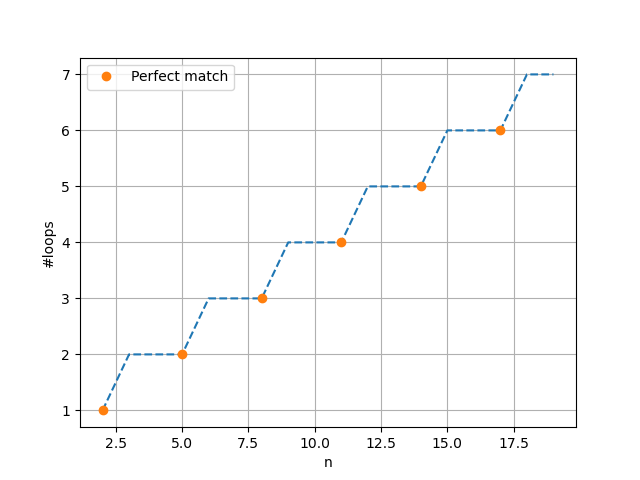
\includegraphics[scale=0.6]{figures/perfect_dim.png}
\end{figure}

This seems to hint that for when $n$ is perfect the amount of information has greater efficiency since in higher dimensions more information can be contained but can be executed in the same number of loops as a non-perfect dim. 
\\ 
The quantum gate $U$ can be formulated as a linear combination of the dark state and dark paths just as in the qutrit case
\begin{equation}
\ket{\psi(t)} = f_0\ket{d} + \sum_{i = 1}^{m}f_i\ket{D_i(t)}, t \in [0,T]
\end{equation}
where the coefficient can be solved for by choosing an initial state $\ket{\psi(0)}$. This corresponds to one loop, by using $\ket{\psi(T)}$ as an initial state for the next loop. By iterating this method one can simulate $\mathbb{U} = U^k$ where each loop $U$ have a different set of parameters. So in theory this can be implemented and simulated for any dimensional qudit, just as for the case of the qutrit. 





